% Figure 2 evidence chain -- generated by
%   experiments/paper/plot_evidence_chain.py --tikz
% Design: docs/figures/FIGURE2_EVIDENCE_CHAIN_GUIDELINE.md
% data source: RQ2=fig6 fp32 values; RQ1=conceptual (rho~0.21, calibrated to 7B); RQ3=conceptual (frozen-op-point infeasible, per alpha_dev_7b)
\definecolor{evGrad}{HTML}{0072B2}
\definecolor{evProx}{HTML}{D55E00}
\definecolor{evMix}{HTML}{009E73}
\definecolor{evCtrl}{HTML}{767676}
\definecolor{evGate}{HTML}{CC79A7}
\definecolor{ink}{HTML}{1A1A1A}
\definecolor{amber}{HTML}{E69F00}
\resizebox{\textwidth}{!}{%
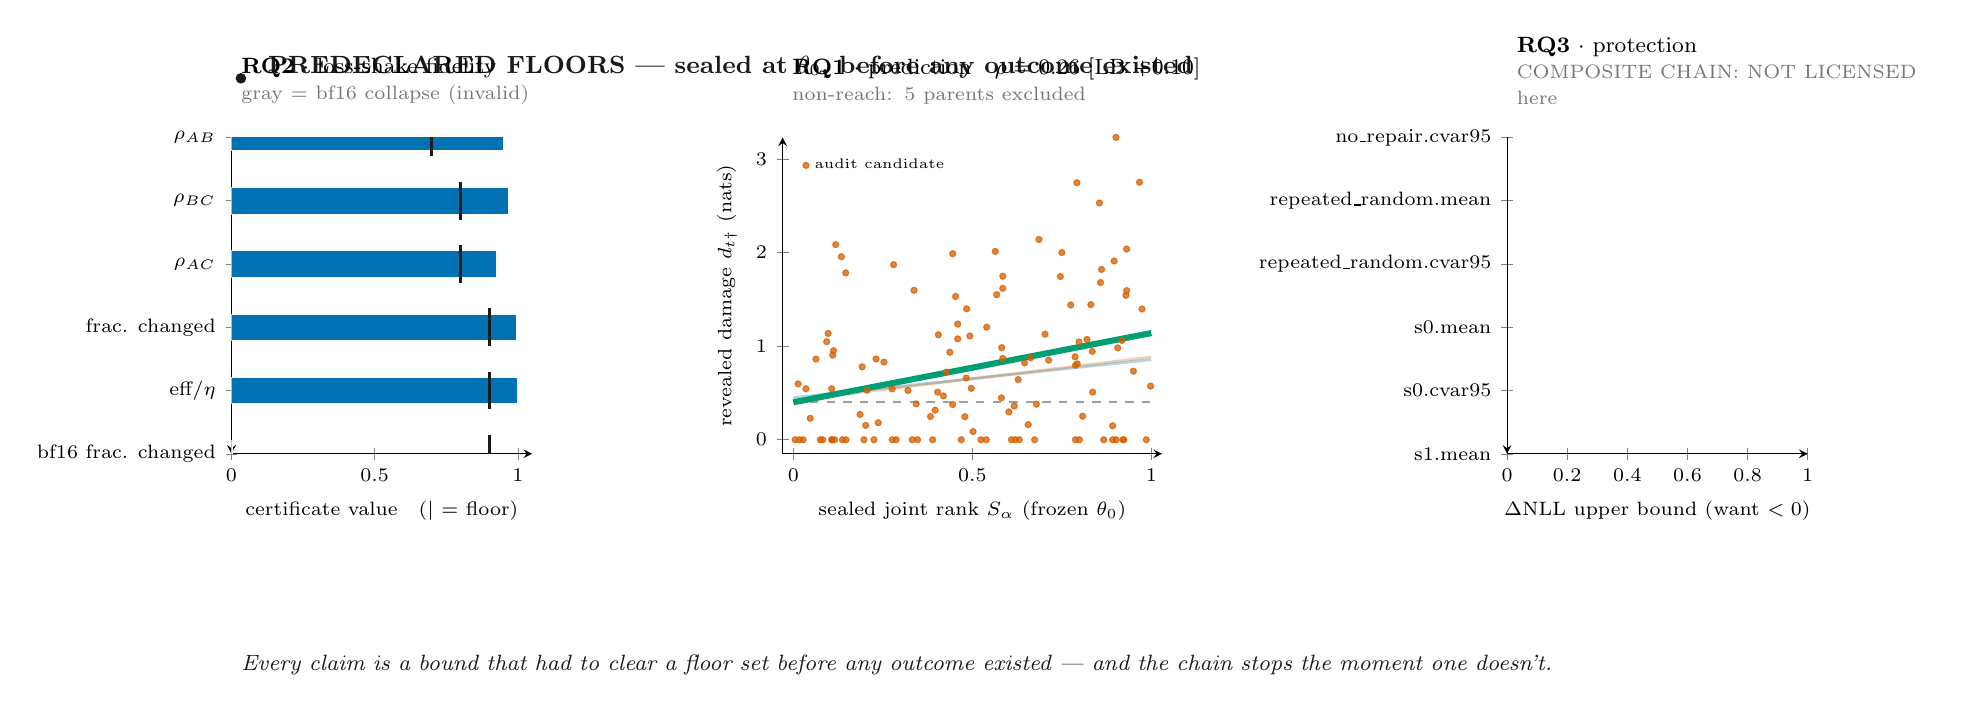
\begin{tikzpicture}[font=\small]
\filldraw[ink] (0.12cm,7.75cm) circle (1.7pt);
\node[anchor=south west, font=\small\bfseries, text=ink] at (0.34cm,7.63cm) {PREDECLARED FLOORS --- sealed at $\theta_0$, before any outcome existed};
\begin{axis}[at={(0.0cm,7.0cm)}, anchor=north west, width=5.4cm, height=5.6cm,
  axis lines=left, y dir=reverse, xmin=0, xmax=1.05,
  title={\textbf{RQ2} $\cdot$ loss-shake fidelity\\\textcolor{evCtrl}{\scriptsize gray = bf16 collapse (invalid)}},
  title style={font=\footnotesize, align=left, text width=5.3cm, at={(0,1.02)}, anchor=south west},
  ytick={0,1,2,3,4,5},
  yticklabels={{$\rho_{AB}$},{$\rho_{BC}$},{$\rho_{AC}$},{frac. changed},{eff$/\eta$},{bf16 frac. changed}},
  yticklabel style={font=\scriptsize}, tick label style={font=\scriptsize},
  xlabel={certificate value \; ($|$ = floor)}, xlabel style={font=\scriptsize}]
\addplot[xbar, bar width=0.42, fill=evGrad, draw=white, line width=0.3pt] coordinates {(0.9506,0)};
\draw[ink, line width=1.1pt] (axis cs:0.7,-0.3) -- (axis cs:0.7,0.3);
\addplot[xbar, bar width=0.42, fill=evGrad, draw=white, line width=0.3pt] coordinates {(0.9657,1)};
\draw[ink, line width=1.1pt] (axis cs:0.8,0.7) -- (axis cs:0.8,1.3);
\addplot[xbar, bar width=0.42, fill=evGrad, draw=white, line width=0.3pt] coordinates {(0.9247,2)};
\draw[ink, line width=1.1pt] (axis cs:0.8,1.7) -- (axis cs:0.8,2.3);
\addplot[xbar, bar width=0.42, fill=evGrad, draw=white, line width=0.3pt] coordinates {(0.9965,3)};
\draw[ink, line width=1.1pt] (axis cs:0.9,2.7) -- (axis cs:0.9,3.3);
\addplot[xbar, bar width=0.42, fill=evGrad, draw=white, line width=0.3pt] coordinates {(1.0000,4)};
\draw[ink, line width=1.1pt] (axis cs:0.9,3.7) -- (axis cs:0.9,4.3);
\addplot[xbar, bar width=0.42, fill=evCtrl, draw=white, line width=0.3pt] coordinates {(0.0019,5)};
\draw[ink, line width=1.1pt] (axis cs:0.9,4.7) -- (axis cs:0.9,5.3);
\end{axis}
\begin{axis}[at={(7.0cm,7.0cm)}, anchor=north west, width=6.4cm, height=5.6cm,
  axis lines=left, xmin=-0.03, xmax=1.03, ymin=-0.15,
  title={\textbf{RQ1} $\cdot$ prediction\quad $\rho=0.26$ [LB $+0.10$]\\\textcolor{evCtrl}{\scriptsize non-reach: 5 parents excluded}},
  title style={font=\footnotesize, align=left, text width=6.3cm, at={(0,1.02)}, anchor=south west},
  xlabel={sealed joint rank $S_\alpha$ (frozen $\theta_0$)},
  ylabel={revealed damage $d_{t\dagger}$ (nats)},
  xlabel style={font=\scriptsize}, ylabel style={font=\scriptsize}, tick label style={font=\scriptsize},
  legend style={font=\tiny, at={(0.03,0.97)}, anchor=north west, draw=none, fill=none}]
\addplot[only marks, mark=*, mark size=1.1pt, color=evProx, opacity=0.75] coordinates {(0.998,0.573) (0.082,0.000) (0.063,0.862) (0.585,1.748) (0.405,1.122) (0.075,0.000) (0.118,2.085) (0.332,0.000) (0.808,0.252) (0.459,1.078) (0.383,0.248) (0.581,0.448) (0.453,1.531) (0.628,0.643) (0.479,0.246) (0.047,0.229) (0.602,0.298) (0.703,1.128) (0.110,0.904) (0.831,1.444) (0.788,0.795) (0.192,0.779) (0.343,0.384) (0.906,0.982) (0.617,0.361) (0.713,0.850) (0.896,1.910) (0.798,1.044) (0.631,0.000) (0.483,0.660) (0.445,0.377) (0.967,2.752) (0.539,0.000) (0.347,0.000) (0.663,0.876) (0.921,0.000) (0.134,1.956) (0.950,0.733) (0.540,1.203) (0.902,0.000) (0.923,0.000) (0.287,0.000) (0.107,0.545) (0.788,0.000) (0.337,1.597) (0.568,1.550) (0.097,1.136) (0.787,0.886) (0.986,0.000) (0.892,0.000) (0.005,0.000) (0.929,1.543) (0.427,0.722) (0.892,0.149) (0.835,0.944) (0.836,0.508) (0.403,0.509) (0.112,0.952) (0.225,0.000) (0.197,0.000) (0.389,0.000) (0.017,0.000) (0.502,0.088) (0.931,1.594) (0.497,0.549) (0.231,0.863) (0.276,0.000) (0.419,0.469) (0.820,1.072) (0.147,0.000) (0.793,0.811) (0.750,2.001) (0.320,0.527) (0.585,0.869) (0.206,0.530) (0.445,1.988) (0.459,1.236) (0.901,3.231) (0.186,0.270) (0.202,0.153) (0.484,1.399) (0.582,0.984) (0.646,0.821) (0.585,1.618) (0.469,0.000) (0.027,0.000) (0.107,0.000) (0.253,0.830) (0.974,1.397) (0.013,0.597) (0.146,1.783) (0.108,0.000) (0.396,0.316) (0.861,1.820) (0.137,0.000) (0.799,0.000) (0.115,0.000) (0.792,2.746) (0.493,1.109) (0.855,2.530) (0.280,1.871) (0.679,0.380) (0.931,2.038) (0.620,0.000) (0.746,1.744) (0.564,2.012) (0.775,1.440) (0.035,0.545) (0.524,0.000) (0.237,0.182) (0.437,0.935) (0.093,1.048) (0.858,1.680) (0.609,0.000) (0.674,0.000) (0.656,0.162) (0.276,0.543) (0.686,2.140) (0.918,1.061) (0.867,0.000)};
\addplot[evGrad, line width=1.0pt, opacity=0.30, forget plot] coordinates {(0,0.450) (1,0.856)};
\addplot[evProx, line width=1.0pt, opacity=0.30, forget plot] coordinates {(0,0.420) (1,0.884)};
\addplot[evCtrl, line width=0.8pt, dashed, opacity=0.7, forget plot] coordinates {(0,0.400) (1,0.400)};
\addplot[evMix, line width=2.2pt, forget plot] coordinates {(0,0.400) (1,1.140)};
\legend{audit candidate}
\end{axis}
\begin{axis}[at={(16.2cm,7.0cm)}, anchor=north west, width=5.4cm, height=5.6cm,
  axis lines=left, y dir=reverse, xmin=-0.26, xmax=0.20,
  title={\textbf{RQ3} $\cdot$ protection\\\textcolor{evCtrl}{\scriptsize COMPOSITE CHAIN: NOT LICENSED here}},
  title style={font=\footnotesize, align=left, text width=5.3cm, at={(0,1.02)}, anchor=south west},
  ytick={0,1,2,3,4,5,6,7},
  yticklabels={{\scriptsize no\_repair.mean},{\scriptsize no\_repair.cvar95},{\scriptsize repeated\_random.mean},{\scriptsize repeated\_random.cvar95},{\scriptsize s0.mean},{\scriptsize s0.cvar95},{\scriptsize s1.mean},{\scriptsize s1.cvar95}},
  tick label style={font=\scriptsize},
  xlabel={$\Delta$NLL upper bound (want $<0$)}, xlabel style={font=\scriptsize}]
\draw[ink, line width=1.2pt] (axis cs:0,-0.6) -- (axis cs:0,7.6);
\draw[evMix, line width=2.6pt] (axis cs:-0.232,0) -- (axis cs:0.000,0);
\filldraw[evMix] (axis cs:-0.232,0) circle (2.4pt);
\draw[evMix, line width=2.6pt] (axis cs:-0.216,1) -- (axis cs:0.000,1);
\filldraw[evMix] (axis cs:-0.216,1) circle (2.4pt);
\draw[evMix, line width=2.6pt] (axis cs:-0.098,2) -- (axis cs:0.000,2);
\filldraw[evMix] (axis cs:-0.098,2) circle (2.4pt);
\draw[evMix, line width=2.6pt] (axis cs:-0.085,3) -- (axis cs:0.000,3);
\filldraw[evMix] (axis cs:-0.085,3) circle (2.4pt);
\draw[evMix, line width=2.6pt] (axis cs:-0.161,4) -- (axis cs:0.000,4);
\filldraw[evMix] (axis cs:-0.161,4) circle (2.4pt);
\draw[evMix, line width=2.6pt] (axis cs:-0.140,5) -- (axis cs:0.000,5);
\filldraw[evMix] (axis cs:-0.140,5) circle (2.4pt);
\draw[evMix, line width=2.6pt] (axis cs:-0.168,6) -- (axis cs:0.000,6);
\filldraw[evMix] (axis cs:-0.168,6) circle (2.4pt);
\draw[evCtrl, line width=0.8pt, dashed] (axis cs:0,7) -- (axis cs:0.110,7);
\filldraw[evCtrl] (axis cs:0.110,7) circle (2.4pt);
\node[anchor=west, font=\tiny, text=evCtrl] at (axis cs:0.110,7) {\; infeasible};
\end{axis}
\node[anchor=north west, font=\footnotesize\itshape, text=ink, text width=21.1cm] at (0cm,0.55cm) {Every claim is a bound that had to clear a floor set before any outcome existed --- and the chain stops the moment one doesn't.};
\end{tikzpicture}%
}
